
%%--------------------------------------------------
%% Serway: Physics for Scientists and Engineers
%%--------------------------------------------------


%% Chapter 13: Universal Gravitation
%%--------------------------------------------------


%% Table of Contents
%%--------------------------------------------------

%% 13.1 Newton's Law of Universal Gravitation
%% 13.2 Free-Fall Acceleration and the Gravitational Force
%% 13.3 Kepler's Laws and the Motion of Planets
%% 13.4 The Gravitational Field
%% 13.5 Gravitational Potential Energy
%% 13.6 Energy Considerations in Planetary and Satellite Motion


%% Serway Multiple Choice Questions
%%--------------------------------------------------
\element{serway-mc}{
\begin{question}{serway-ch13-q01}
    A satellite circles planet Roton every \SI{2.8}{\hour} in an orbit having a radius of \SI{1.2e7}{\meter}.
    If the radius of Roton is \SI{5.0e6}{\meter},
        what is the magnitude of the free-fall acceleration on the surface of Roton?
    \begin{multicols}{3}
    \begin{choices}
        \wrongchoice{\SI{31}{\meter\per\second\squared}}
      \correctchoice{\SI{27}{\meter\per\second\squared}}
        \wrongchoice{\SI{34}{\meter\per\second\squared}}
        \wrongchoice{\SI{40}{\meter\per\second\squared}}
        \wrongchoice{\SI{19}{\meter\per\second\squared}}
    \end{choices}
    \end{multicols}
\end{question}
}

\element{serway-mc}{
\begin{question}{serway-ch13-q02}
    The period of a satellite circling planet Nutron is observed to be \SI{84}{\second} when it is in a circular orbit with a radius of \SI{8.0e6}{\meter}.
    What is the mass of planet Nutron?
    \begin{multicols}{2}
    \begin{choices}
        \wrongchoice{\SI{6.2e28}{\kilo\gram}}
        \wrongchoice{\SI{5.0e28}{\kilo\gram}}
        \wrongchoice{\SI{5.5e28}{\kilo\gram}}
      \correctchoice{\SI{4.3e28}{\kilo\gram}}
        \wrongchoice{\SI{3.7e28}{\kilo\gram}}
    \end{choices}
    \end{multicols}
\end{question}
}

\element{serway-mc}{
\begin{question}{serway-ch13-q03}
    A \SI{50}{\kilo\gram} satellite circles planet Cruton every \SI{5.6}{\hour} in an orbit with a radius of \SI{12e6}{\meter}.
    What is the magnitude of the gravitational force on the satellite by planet Cruton?
    \begin{multicols}{3}
    \begin{choices}
        \wrongchoice{\SI{63}{\newton}}
      \correctchoice{\SI{58}{\newton}}
        \wrongchoice{\SI{68}{\newton}}
        \wrongchoice{\SI{73}{\newton}}
        \wrongchoice{\SI{50}{\newton}}
    \end{choices}
    \end{multicols}
\end{question}
}

\element{serway-mc}{
\begin{question}{serway-ch13-q04}
    Two stars of masses $M$ and $6M$ are separated by a distance $D$.
    Determine the distance (measured from $M$)
        to a point at which the net gravitational force on a third mass would be zero.
    \begin{multicols}{3}
    \begin{choices}
        \wrongchoice{$0.41 D$}
        \wrongchoice{$0.33 D$}
        \wrongchoice{$0.37 D$}
      \correctchoice{$0.29 D$}
        \wrongchoice{$0.14 D$}
    \end{choices}
    \end{multicols}
\end{question}
}

\element{serway-mc}{
\begin{question}{serway-ch13-q05}
    What is the magnitude of the free-fall acceleration at a point that is a distance $2R$ above the surface of the Earth,
        where $R$ is the radius of the Earth?
    \begin{multicols}{2}
    \begin{choices}
        \wrongchoice{\SI{4.8}{\meter\per\second\squared}}
      \correctchoice{\SI{1.1}{\meter\per\second\squared}}
        \wrongchoice{\SI{3.3}{\meter\per\second\squared}}
        \wrongchoice{\SI{2.5}{\meter\per\second\squared}}
        \wrongchoice{\SI{6.5}{\meter\per\second\squared}}
    \end{choices}
    \end{multicols}
\end{question}
}

\element{serway-mc}{
\begin{question}{serway-ch13-q06}
    A satellite is in a circular orbit about the Earth at an altitude at which air resistance is negligible.
    Which of the following statements is true?
    \begin{choices}
      \correctchoice{There is only one force acting on the satellite.}
        \wrongchoice{There are two forces acting on the satellite, and their resultant is zero.}
        \wrongchoice{There are two forces acting on the satellite, and their resultant is not zero.}
        \wrongchoice{There are three forces acting on the satellite.}
        \wrongchoice{None of the preceding statements are correct.}
    \end{choices}
\end{question}
}

\newcommand{\serwayChThirteenQSeven}{
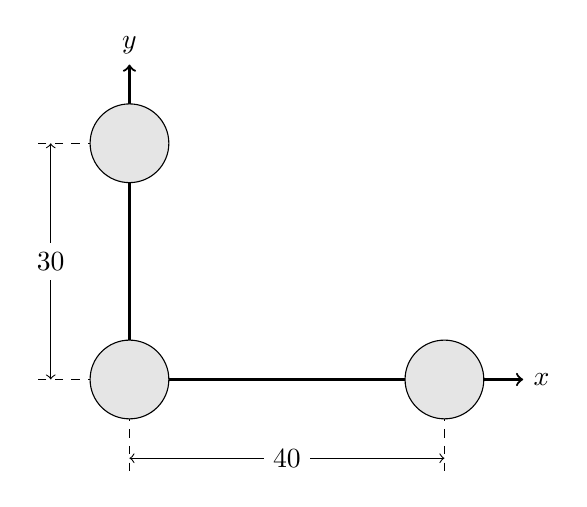
\begin{tikzpicture}
    %% x and y axis
    \draw[thick,->] (0,0) -- (0,4) node[anchor=south] {$y$};
    \draw[thick,->] (0,0) -- (5,0) node[anchor=west] {$x$};
    \draw[dashed] (0,0) -- (-1.25,0);
    \draw[dashed] (0,3) -- (-1.25,3);
    \draw[dashed] (0,0) -- (0,-1.25);
    \draw[dashed] (4,0) -- (4,-1.25);
    %% three masses
    \draw[fill=white!90!black] (0,3) circle (0.5cm);
    \draw[fill=white!90!black] (0,0) circle (0.5cm);
    \draw[fill=white!90!black] (4,0) circle (0.5cm);
    %% width and length
    \draw[<->] (-1,0) -- (-1,3) node[pos=0.5,anchor=center,fill=white] {\SI{30}{\centi\meter}};
    \draw[<->] (0,-1) -- (4,-1) node[pos=0.5,anchor=center,fill=white] {\SI{40}{\centi\meter}};
\end{tikzpicture}
}

\element{serway-mc}{
\begin{question}{serway-ch13-q07}
    Three \SI{5.0}{\kilo\gram} masses are located at points in the $xy$ plane as shown in the figure.
    \begin{center}
        \serwayChThirteenQSeven
    \end{center}
    What is the magnitude of the resultant force
        (caused by the other two masses) on the mass at the origin?
    \begin{multicols}{2}
    \begin{choices}
        \wrongchoice{\SI{2.7e-8}{\newton}}
      \correctchoice{\SI{2.1e-8}{\newton}}
        \wrongchoice{\SI{1.8e-8}{\newton}}
        \wrongchoice{\SI{2.4e-8}{\newton}}
        \wrongchoice{\SI{2.9e-8}{\newton}}
    \end{choices}
    \end{multicols}
\end{question}
}

\element{serway-mc}{
\begin{question}{serway-ch13-q08}
    Three \SI{5.0}{\kilo\gram} masses are located at points in the xy plane, as shown.
    \begin{center}
        \serwayChThirteenQSeven
    \end{center}
    What is the magnitude of the resultant force   
        (caused by the other two masses) on the mass at $x=\SI{0.40}{\meter}$, $y=\SI{0}{\meter}$?
    \begin{multicols}{2}
    \begin{choices}
        \wrongchoice{\SI{2.2e-8}{\newton}}
        \wrongchoice{\SI{1.9e-8}{\newton}}
        \wrongchoice{\SI{1.4e-8}{\newton}}
      \correctchoice{\SI{1.6e-8}{\newton}}
        \wrongchoice{\SI{2.5e-8}{\newton}}
    \end{choices}
    \end{multicols}
\end{question}
}

\element{serway-mc}{
\begin{question}{serway-ch13-q09}
    Three \SI{5.0}{\kilo\gram} masses are located at points in the xy plane, as shown.
    \begin{center}
        %% original uses m instead of cm
        \serwayChThirteenQSeven
    \end{center}
    What is the magnitude of the resultant force   
        (caused by the other two masses) on the mass at $x=\SI{0}{\meter}$, $y=\SI{0.30}{\meter}$?
    \begin{multicols}{2}
    \begin{choices}
        \wrongchoice{\SI{2.6e-8}{\newton}}
        \wrongchoice{\SI{2.0e-8}{\newton}}
        \wrongchoice{\SI{2.9e-8}{\newton}}
      \correctchoice{\SI{2.3e-8}{\newton}}
        \wrongchoice{\SI{2.1e-8}{\newton}}
    \end{choices}
    \end{multicols}
\end{question}
}

\element{serway-mc}{
\begin{question}{serway-ch13-q10}
    What is the gravitational force on a \SI{20}{\kilo\gram} satellite circling the Earth
        (radius = \SI{6.4e6}{\meter}, mass = \SI{6.0e24}{\kilo\gram}) with a period of \SI{5.0}{\hour}?
    \begin{multicols}{3}
    \begin{choices}
        \wrongchoice{\SI{88}{\newton}}
        \wrongchoice{\SI{55}{\newton}}
      \correctchoice{\SI{36}{\newton}}
        \wrongchoice{\SI{98}{\newton}}
        \wrongchoice{\SI{18}{\newton}}
    \end{choices}
    \end{multicols}
\end{question}
}

\element{serway-mc}{
\begin{question}{serway-ch13-q11}
    A spaceship of mass $m$ circles a planet (mass = $M$) in an orbit of radius $R$.
    How much energy is required to transfer the spaceship to a circular orbit of radius $3R$?
    \begin{multicols}{3}
    \begin{choices}
        \wrongchoice{$\dfrac{GmM}{2R}$}
      \correctchoice{$\dfrac{GmM}{3R}$}
        \wrongchoice{$\dfrac{GmM}{4R}$}
        \wrongchoice{$\dfrac{GmM}{6R}$}
        \wrongchoice{$\dfrac{3GmM}{4R}$}
    \end{choices}
    \end{multicols}
\end{question}
}

\element{serway-mc}{
\begin{question}{serway-ch13-q12}
    A spacecraft (mass = $m$) orbits a planet (mass = $M$) in a circular orbit (radius = $R$).
    What is the minimum energy required to send this spacecraft to a distant
        point in space where the gravitational force on the spacecraft by the planet is negligible?
    \begin{multicols}{3}
    \begin{choices}
        \wrongchoice{$\dfrac{GmM}{4R}$}
        \wrongchoice{$\dfrac{GmM}{R}$}
      \correctchoice{$\dfrac{GmM}{2R}$}
        \wrongchoice{$\dfrac{GmM}{3R}$}
        \wrongchoice{$\dfrac{2GmM}{5R}$}
    \end{choices}
    \end{multicols}
\end{question}
}

\element{serway-mc}{
\begin{question}{serway-ch13-q13}
    A projectile is launched from the surface of a planet (mass = $M$, radius = $R$).
    What minimum launch speed is required if the projectile is to rise to a height of $2R$ above the surface of the planet?
    Disregard any dissipative effects of the atmosphere.
    \begin{multicols}{3}
    \begin{choices}
      \correctchoice{$\sqrt{\dfrac{4GmM}{3R}}$}
        \wrongchoice{$\sqrt{\dfrac{8GmM}{5R}}$}
        \wrongchoice{$\sqrt{\dfrac{3GmM}{2R}}$}
        \wrongchoice{$\sqrt{\dfrac{5GmM}{3R}}$}
        \wrongchoice{$\sqrt{\dfrac{GmM}{3R}}$}
    \end{choices}
    \end{multicols}
\end{question}
}

\element{serway-mc}{
\begin{question}{serway-ch13-q14}
    An object is released from rest at a distance $h$ above the surface of a planet
        (mass = $M$, radius = $R<h$).
    With what speed will the object strike the surface of the planet?
    Disregard any dissipative effects of the atmosphere of the planet.
    \begin{multicols}{2}
    \begin{choices}
      \correctchoice{$\sqrt{\dfrac{2GmMh}{R\left(R+H\right)}}$}
        \wrongchoice{$\sqrt{\dfrac{2GmM}{R}}$}
        \wrongchoice{$\sqrt{\dfrac{3GmM\left(h-R\right)}{Rh}}$}
        \wrongchoice{$\sqrt{\dfrac{2GmM}{R+h}}$}
        \wrongchoice{$\sqrt{\dfrac{2GmM}{R+h}}$}
    \end{choices}
    \end{multicols}
\end{question}
}

\element{serway-mc}{
\begin{question}{serway-ch13-q15}
    What is the kinetic energy of a \SI{200}{\kilo\gram} satellite as it follows a circular orbit of radius \SI{8.0e6}{\meter} around the Earth?
    (Mass of Earth = \SI{6.0e24}{\kilo\gram}.)
    \begin{multicols}{2}
    \begin{choices}
      \correctchoice{\SI{5.0e9}{\joule}}
        \wrongchoice{\SI{1.0e10}{\joule}}
        \wrongchoice{\SI{1.5e10}{\joule}}
        \wrongchoice{\SI{2.0e10}{\joule}}
        \wrongchoice{\SI{2.5e9}{\joule}}
    \end{choices}
    \end{multicols}
\end{question}
}

\element{serway-mc}{
\begin{question}{serway-ch13-q16}
    An object is released from rest when it is a height $h$ above the surface of a planet of mass $M$ and radius $R$.
    What is the speed of the object just before striking the surface of the planet?
    Neglect any air resistance.
    Let $h=\SI{4.0e6}{\meter}$, $R=\SI{5.0e6}{\meter}$, and $M=\SI{4.0e24}{\kilo\gram}$.
    \begin{multicols}{2}
    \begin{choices}
        \wrongchoice{\SI{7.8}{\kilo\meter\per\second}}
        \wrongchoice{\SI{3.5}{\kilo\meter\per\second}}
        \wrongchoice{\SI{5.4}{\kilo\meter\per\second}}
      \correctchoice{\SI{6.9}{\kilo\meter\per\second}}
        \wrongchoice{\SI{4.8}{\kilo\meter\per\second}}
    \end{choices}
    \end{multicols}
\end{question}
}

\element{serway-mc}{
\begin{question}{serway-ch13-q17}
    A \SI{50}{\kilo\gram} satellite circles the Earth in an orbit with a period of \SI{120}{\minute}.
    What minimum energy is required to change the orbit to another circular orbit with a period of \SI{180}{\minute}?
    (Earth: radius = \SI{6.4e6}{\meter}, mass = \SI{6.0e24}{\kilo\gram})
    \begin{multicols}{2}
    \begin{choices}
      \correctchoice{\SI{2.9e8}{\joule}}
        \wrongchoice{\SI{3.5e8}{\joule}}
        \wrongchoice{\SI{4.1e8}{\joule}}
        \wrongchoice{\SI{4.7e8}{\joule}}
        \wrongchoice{\SI{5.9e8}{\joule}}
    \end{choices}
    \end{multicols}
\end{question}
}

\element{serway-mc}{
\begin{question}{serway-ch13-q18}
    Planet Roton has a mass of \SI{4.0e23}{\kilo\gram} and a radius of \SI{2.0e6}{\meter}.
    With what speed should a space probe be launched from the surface of Roton so as to achieve a maximum distance of \SI{3.0e6}{\meter} from the center of Roton?
    \begin{multicols}{2}
    \begin{choices}
        \wrongchoice{\SI{4.2}{\kilo\meter\per\second}}
        \wrongchoice{\SI{3.9}{\kilo\meter\per\second}}
      \correctchoice{\SI{3.0}{\kilo\meter\per\second}}
        \wrongchoice{\SI{3.4}{\kilo\meter\per\second}}
        \wrongchoice{\SI{6.0}{\kilo\meter\per\second}}
    \end{choices}
    \end{multicols}
\end{question}
}

\element{serway-mc}{
\begin{question}{serway-ch13-q19}
    Planet Zero has a mass of \SI{5.0e23}{\kilo\gram} and a radius of \SI{2.0e6}{\meter}.
    A space probe is launched vertically from the surface of Zero with an initial speed of \SI{4.0}{\kilo\meter\per\second}.
    What is the speed of the probe when it is \SI{3.0e6}{\meter} from Zero’s center?
    \begin{multicols}{2}
    \begin{choices}
        \wrongchoice{\SI{3.0}{\kilo\meter\per\second}}
      \correctchoice{\SI{2.2}{\kilo\meter\per\second}}
        \wrongchoice{\SI{1.6}{\kilo\meter\per\second}}
        \wrongchoice{\SI{3.7}{\kilo\meter\per\second}}
        \wrongchoice{\SI{5.9}{\kilo\meter\per\second}}
    \end{choices}
    \end{multicols}
\end{question}
}

\element{serway-mc}{
\begin{question}{serway-ch13-q20}
    What is the escape speed from a planet of mass $M$ and radius $R$ if $M=\SI{3.2e23}{\kilo\gram}$ and $R=\SI{2.4e6}{\meter}$?
    \begin{multicols}{2}
    \begin{choices}
        \wrongchoice{\SI{5.5}{\kilo\meter\per\second}}
      \correctchoice{\SI{4.2}{\kilo\meter\per\second}}
        \wrongchoice{\SI{5.2}{\kilo\meter\per\second}}
        \wrongchoice{\SI{4.8}{\kilo\meter\per\second}}
        \wrongchoice{\SI{3.7}{\kilo\meter\per\second}}
    \end{choices}
    \end{multicols}
\end{question}
}

\element{serway-mc}{
\begin{question}{serway-ch13-q21}
    A satellite of mass $m$ circles a planet of mass $M$ and radius $R$ in an orbit at a height $2R$ above the surface of the planet.
    What minimum energy is required to change the orbit to one for which the height of the satellite is $3R$ above the surface of the planet?
    \begin{multicols}{3}
    \begin{choices}
      \correctchoice{$\dfrac{GmM}{24 R}$}
        \wrongchoice{$\dfrac{GmM}{15 R}$}
        \wrongchoice{$\dfrac{GmM}{12 R}$}
        \wrongchoice{$\dfrac{2 GmM}{21 R}$}
        \wrongchoice{$\dfrac{3 GmM}{5 R}$}
    \end{choices}
    \end{multicols}
\end{question}
}

\element{serway-mc}{
\begin{question}{serway-ch13-q22}
    Planet Zero has a mass of \SI{4.0e23}{\kilo\gram} and a radius of \SI{2.0e6}{\meter}.
    A \SI{10}{\kilo\gram} space probe is launched vertically from the surface of Zero with an initial kinetic energy of \SI{8.0e7}{\joule}.
    What maximum distance from the center of Zero is achieved by the probe?
    \begin{multicols}{2}
    \begin{choices}
        \wrongchoice{\SI{3.2e6}{\meter}}
        \wrongchoice{\SI{4.0e6}{\meter}}
        \wrongchoice{\SI{6.0e6}{\meter}}
      \correctchoice{\SI{5.0e6}{\meter}}
        \wrongchoice{\SI{2.5e6}{\meter}}
    \end{choices}
    \end{multicols}
\end{question}
}

\element{serway-mc}{
\begin{question}{serway-ch13-q23}
    Two satellites are placed in geosynchronous orbits,
        orbits with a period of 24 hours,
        where each satellite hovers over a spot on the Earth's equator.
    Satellite $B$ has three times the mass of satellite $A$.
    What is the relationship between the magnitudes of the
        gravitational forces of the Earth on the two satellites?
    \begin{multicols}{2}
    \begin{choices}
        \wrongchoice{$F_B = \dfrac{1}{9} F_A$}
        \wrongchoice{$F_B = \dfrac{1}{3} F_A$}
        \wrongchoice{$F_B = F_A$}
      \correctchoice{$F_B = 3F_A$}
        \wrongchoice{$F_B = 9F_A$}
    \end{choices}
    \end{multicols}
\end{question}
}

\element{serway-mc}{
\begin{question}{serway-ch13-q24}
    A satellite is placed in a geosynchronous orbit.
    In this equatorial orbit with a period of 24 hours,
        the satellite hovers over one point on the equator.
    Which statement is true for a satellite in such an orbit?
    \begin{choices}
        \wrongchoice{There is no gravitational force on the satellite.}
        \wrongchoice{There is no acceleration toward the center of the Earth.}
      \correctchoice{The satellite is in a state of free fall toward the Earth.}
        \wrongchoice{There is a tangential force that helps the satellite keep up with the rotation of the Earth.}
        \wrongchoice{The force toward the center of the Earth is balanced by a force away from the center of the Earth.}
    \end{choices}
\end{question}
}

\element{serway-mc}{
\begin{question}{serway-ch13-q25}
    Two identical planets orbit a star in concentric circular orbits in the star's equatorial plane. Of the two, the planet that is farther from the star must have:
    \begin{choices}
        \wrongchoice{the smaller period.}
      \correctchoice{the greater period.}
        \wrongchoice{the smaller gravitational mass.}
        \wrongchoice{the larger gravitational mass.}
        \wrongchoice{the larger universal gravitational constant.}
    \end{choices}
\end{question}
}

\element{serway-mc}{
\begin{question}{serway-ch13-q26}
    Which of the following quantities is conserved for a planet orbiting a star in a circular orbit?
    Only the planet itself is to be taken as the system;
        the star is not included.
    \begin{choices}
        \wrongchoice{Momentum and energy.}
      \correctchoice{Energy and angular momentum.}
        \wrongchoice{Momentum and angular momentum.}
        \wrongchoice{Momentum, angular momentum and energy.}
        \wrongchoice{None of the above.}
    \end{choices}
\end{question}
}

\newcommand{\serwayChThirteenQTwentySeven}{
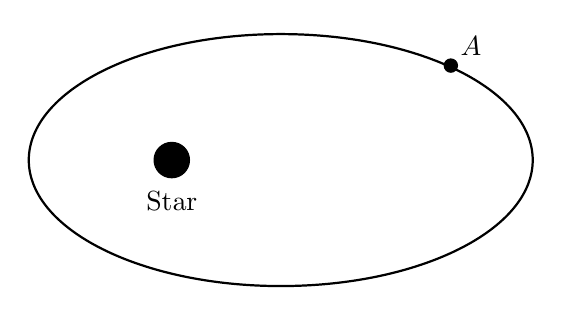
\begin{tikzpicture}[scale=0.8]
    %% orbit and center
    \draw[thick] (0,0) circle (4cm and 2cm);
    \draw[fill] (-1.73,0) circle (8pt) node[anchor=north,yshift=-8pt] {Star};
    %% diagonals (trial and error)
    \draw[fill] (+2.7,+1.5) circle (3pt) node[anchor=south west] {$A$};
\end{tikzpicture}
}

\element{serway-mc}{
\begin{question}{serway-ch13-q27}
    The figure below shows a planet traveling in a counterclockwise direction on an elliptical path around a star located at one focus of the ellipse.
    \begin{center}
        \serwayChThirteenQTwentySeven
    \end{center}
    When the planet is at point $A$,
    \begin{choices}
        \wrongchoice{its speed is constant.}
      \correctchoice{its speed is increasing.}
        \wrongchoice{its speed is decreasing.}
        \wrongchoice{its speed is a maximum.}
        \wrongchoice{its speed is a minimum.}
    \end{choices}
\end{question}
}

\element{serway-mc}{
\begin{question}{serway-ch13-q28}
    The figure below shows a planet traveling in a clockwise direction on an elliptical path around a star located at one focus of the ellipse.
    \begin{center}
        \serwayChThirteenQTwentySeven
    \end{center}
    When the planet is at point $A$,
    \begin{choices}
        \wrongchoice{its speed is constant.}
        \wrongchoice{its speed is increasing.}
      \correctchoice{its speed is decreasing.}
        \wrongchoice{its speed is a maximum.}
        \wrongchoice{its speed is a minimum.}
    \end{choices}
\end{question}
}

\element{serway-mc}{
\begin{question}{serway-ch13-q29}
    The figure below shows a planet traveling in a counterclockwise direction on an elliptical path around a star located at one focus of the ellipse.
    \begin{center}
    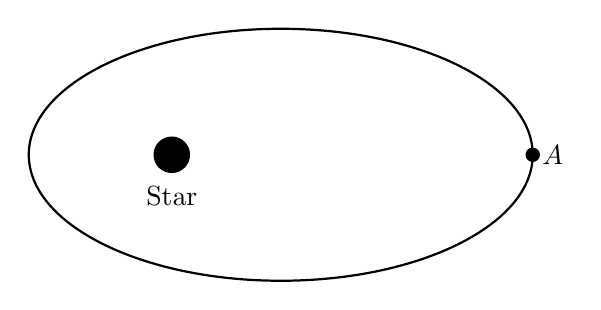
\begin{tikzpicture}[scale=0.8]
        %% orbit and center
        \draw[thick] (0,0) circle (4cm and 2cm);
        \draw[fill] (-1.73,0) circle (8pt) node[anchor=north,yshift=-8pt] {Star};
        %% Left and right
        \draw[fill] (+4,0) circle (3pt) node[anchor=west] {$A$};
    \end{tikzpicture}
    \end{center}
    When the planet is at point $A$,
    \begin{choices}
        \wrongchoice{its speed is constant.}
        \wrongchoice{its speed is increasing.}
        \wrongchoice{its speed is decreasing.}
        \wrongchoice{its speed is a maximum.}
      \correctchoice{its speed is a minimum.}
    \end{choices}
\end{question}
}

\newcommand{\serwayChThirteenQThirty}{
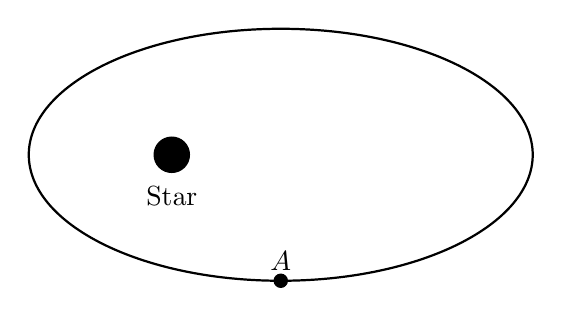
\begin{tikzpicture}[scale=0.8]
    %% orbit and center
    \draw[thick] (0,0) circle (4cm and 2cm);
    \draw[fill] (-1.73,0) circle (8pt) node[anchor=north,yshift=-8pt] {Star};
    %% top and bottom
    \draw[fill] (0,-2) circle (3pt) node[anchor=south] {$A$};
\end{tikzpicture}
}


\element{serway-mc}{
\begin{question}{serway-ch13-q30}
    The figure below shows a planet traveling in a counterclockwise direction on an elliptical path around a star located at one focus of the ellipse.
    \begin{center}
        \serwayChThirteenQThirty
    \end{center}
    When the planet is
    \begin{choices}
        \wrongchoice{its speed is constant.}
        \wrongchoice{its speed is increasing.}
      \correctchoice{its speed is decreasing.}
        \wrongchoice{its speed is a maximum.}
        \wrongchoice{its speed is a minimum.}
    \end{choices}
\end{question}
}

\element{serway-mc}{
\begin{question}{serway-ch13-q31}
    The figure below shows a planet traveling in a clockwise direction on an elliptical path around a star located at one focus of the ellipse.
    \begin{center}
        \serwayChThirteenQThirty
    \end{center}
    When the planet is at point $A$,
    \begin{choices}
        \wrongchoice{its speed is constant.}
      \correctchoice{its speed is increasing.}
        \wrongchoice{its speed is decreasing.}
        \wrongchoice{its speed is a maximum.}
        \wrongchoice{its speed is a minimum.}
    \end{choices}
\end{question}
}

\element{serway-mc}{
\begin{questionmult}{serway-ch13-q32}
    The figure below shows a planet traveling in a counterclockwise direction on an elliptical path around a star located at one focus of the ellipse.
    \begin{center}
        \serwayChThirteenQTwentySeven
    \end{center}
    When the planet is at point $A$,
    \begin{choices}
        \wrongchoice{its speed is decreasing.}
        \wrongchoice{its angular momentum is increasing.}
        \wrongchoice{the gravitational force does no work on the planet..}
        %\wrongchoice{all of the above are correct.}
        %\correctchoice{none of the provided are correct.}
    \end{choices}
\end{questionmult}
}

\element{serway-mc}{
\begin{question}{serway-ch13-q33}
    The period of oscillation of an object in a frictionless tunnel running through the Earth is \SI{84.3}{\minute}.
    What is the period of oscillation of an object in a similar tunnel on the Moon?
    ($R_E=\SI{6.37e6}{\meter}$; $R_M=\SI{1.74e6}{\meter}$;
        $M_E=\SI{5.98e24}{\kilo\gram}$; $M_M=\SI{7.36e22}{\kilo\gram}$.)
    \begin{multicols}{2}
    \begin{choices}
        \wrongchoice{\SI{6.03e-3}{\minute}}
        \wrongchoice{\SI{0.713}{\minute}}
        \wrongchoice{\SI{84.3}{\minute}}
      \correctchoice{\SI{108.5}{\minute}}
        \wrongchoice{\SI{139.6}{\minute}}
    \end{choices}
    \end{multicols}
\end{question}
}

\element{serway-mc}{
\begin{question}{serway-ch13-q34}
    Three galaxies, each of mass $M=\SI{4.0e41}{\kilo\gram}$,
        lie in a plane at the corners of an equilateral triangle with sides of \SI{5.0e22}{\meter} length.
    The magnitude of the force the other two galaxies exert on each galaxy is
    \begin{multicols}{2}
    \begin{choices}
        \wrongchoice{\SI{4.3e27}{\newton}}
        \wrongchoice{\SI{6.4e27}{\newton}}
      \correctchoice{\SI{7.4e27}{\newton}}
        \wrongchoice{\SI{8.6e27}{\newton}}
        \wrongchoice{\SI{4.3e28}{\newton}}
    \end{choices}
    \end{multicols}
\end{question}
}

\element{serway-mc}{
\begin{question}{serway-ch13-q35}
    Knowing that $g=\SI{9.80}{\meter\per\second\squared}$ at sea level and that $R_E=\SI{6.37e6}{\meter}$,
        we find that the value of $g$ at a distance $R_E$ from the surface of the Earth is:
    \begin{multicols}{2}
    \begin{choices}
        \wrongchoice{\SI{1.23}{\meter\per\second\squared}}
      \correctchoice{\SI{2.45}{\meter\per\second\squared}}
        \wrongchoice{\SI{4.90}{\meter\per\second\squared}}
        \wrongchoice{\SI{7.35}{\meter\per\second\squared}}
        \wrongchoice{\SI{9.80}{\meter\per\second\squared}}
    \end{choices}
    \end{multicols}
\end{question}
}

\element{serway-mc}{
\begin{question}{serway-ch13-q36}
    When two solid spheres of the same material and same radius $r$ are in contact,
        the magnitude of the gravitational force each exerts on the other is directly proportional to:
    \begin{multicols}{3}
    \begin{choices}
        \wrongchoice{$r$}
        \wrongchoice{$r^2$}
        \wrongchoice{$r^3$}
      \correctchoice{$r^4$}
        \wrongchoice{$r^6$}
    \end{choices}
    \end{multicols}
\end{question}
}

\element{serway-mc}{
\begin{question}{serway-ch13-q37}
    Huyghens claimed that near the surface of the Earth the velocity downwards of an object released from rest, $v_y$,
        was directly proportional to the square root of the distance it had fallen,
        $v_y = c\sqrt{y}$.
    This is true if $c$ is equal to:
    \begin{multicols}{3}
    \begin{choices}
        \wrongchoice{$\dfrac{g}{4}$}
        \wrongchoice{$\dfrac{g}{2}$}
        \wrongchoice{$g$}
      \correctchoice{$2g$}
        \wrongchoice{$4g$}
    \end{choices}
    \end{multicols}
\end{question}
}

\element{serway-mc}{
\begin{question}{serway-ch13-q38}
    Suppose the gravitational force of the Earth on a body was $F=-\dfrac{KM_E m}{r^3}$.
    What escape velocity $v_e$ would a body need to escape the gravitational field of the Earth?
    \begin{multicols}{2}
    \begin{choices}
        \wrongchoice{$v_e = \sqrt{\dfrac{KM_E}{2R_E^2}}$}
      \correctchoice{$v_e = \sqrt{\dfrac{KM_E}{R_E^2}}$}
        \wrongchoice{$v_e = \sqrt{\dfrac{KM_E}{2 R_E}}$}
        \wrongchoice{$v_e = \sqrt{\dfrac{KM_E}{R_E}}$}
        \wrongchoice{$v_e = \sqrt{KM_E}$}
    \end{choices}
    \end{multicols}
\end{question}
}

\element{serway-mc}{
\begin{questionmult}{serway-ch13-q39}
    In an isolated system of two bodies that exert gravitational forces on one another,
        the quantity (quantities) that remain(s) constant is(are):
    \begin{choices}
      \correctchoice{the total energy of the system.}
      \correctchoice{the total angular momentum of the system.}
        \wrongchoice{the angular positions of the two bodies.}
        %\wrongchoice{all of the above.}
        %\correctchoice{only (a) and (b) above.}
    \end{choices}
\end{questionmult}
}

\element{serway-mc}{
\begin{question}{serway-ch13-q40}
    Carla and Jenny are arguing about whether or not it is possible to escape the gravitational field of the Earth.
    Carla shows Jenny the system below where mass $m$ is $r_E$ (not the Earth's radius) distant from Earth and $r_P$ (not planet $P$'s radius) distant from planet $P$.
    Carla states that the mass $m$ has escaped if $F_{\text{$P$ on $m$}} = -F_{\text{$E$ on $M$}}$.
    Which one, if either, is correct, and why?
    \begin{choices}
        \wrongchoice{Carla, because the total gravitational force on $m$ is zero at that point.}
        \wrongchoice{Carla, because there is no gravitational force from Earth on $m$ at that point.}
        \wrongchoice{Carla, because there is no gravitational force on $m$ from Earth when $r > r_E$.}
      \correctchoice{Jenny, because there is a gravitational force on $m$ from Earth no matter how great the distance from the Earth.}
        \wrongchoice{Jenny, because the gravitational force from the Earth can only be blocked by a body that is larger than the Earth.}
    \end{choices}
\end{question}
}


\endinput



